%% ------------------------------------------------------------------------- %%
\chapter{Evaluations, Results, and Discussion}
\label{cap:evaluations}

%%MQZ: Aqui tem MUITA repetição do capítulo de metodologia! Estou eliminando as redundâncias, mas a fluência do texto será prejudicada...
%% Também não faz sentido no seu capítulo de resultados apresentar resultados de outros (isso fica em "trabalhos relacionados", não aqui...)
%\paragraphdesc{motivation based on experiences from compmus and nusom}
%Currently I am a member of Computer Music Research Group~(Compmus) from Universidade de São Paulo, and this group is a partner of the Research Centre on Sonology~(NuSom) from the same university.
%Recent projects and performances at the Compmus and NuSom research groups have used technologies for music interaction for short and long range distances.
%Scientists and musicians were working together in order to create multimedia environments for musical performances using local networks and the Internet.
%As this research unfolded, mobile devices have reached a comparable level of computation power with respect to desktop computers, having their mobility also improved by advances in network technologies such as the development of 4G and faster WiFi standards.
%The projects from the group and the advances in mobile technologies during the 2010's encouraged the development of this research in the field of music and mobile networks, or better saying in MM.

%\paragraphdesc{group results}
%The past researches decided to transmit audio between devices locally connected or through the Internet, but some researchers were the main inspiration for this work.
%As previously discussed, \citefullauthor{Schiavoni2013thesis} developed Medusa, a distributed audio environment~\cite{Schiavoni2013thesis} that allows users to interconnect using several  network protocols for audio and MIDI exchange.
%The protocols implemented were UDP, TCP, DCCP, and SCTP while the audio transmitted was configured to 44.1~kHz and 16~bits that would require a network bandwidth of almost 700~kbps for each audio channel.
%Many evaluations were conducted in different scenarios for LAN intercommunication, with latency varying from 0.13~ms to 72.06~ms, jitter varying from 0.08~ms to 166.49~ms, and packet loss up to 7.065\%.
%%MQZ: o Marcio não fez avaliações de comunicação em rede.
%Another research is \citefullauthor{Tomiyoshi2013thesis}, who developed the JackTripMod, a flexible and easy-to-use alternative for network music performances~\cite{Tomiyoshi2013thesis}.
%As modification of the JackTrip, this project includes a lossy compression using CELT~\cite{Valin2010high}, which is an efficient and low latency solution for encoding audio before transmitting over the network.
%This project shows that 93~kbps is the bandwidth required for transmitting an audio with 48~kbps of compression quality through the JackTripMod, in comparison with the 128~kbps required by the SoundJack~\cite{Carot2009musical} at the same setting and the 28~kbps by Skype~\cite{Skype2017} with an unknown configuration.
%Their results show that some protocols have good performance for local audio transmission in local networks, and audio transmission with lossy compression and high quality is possible depending on the network bandwidth available.
%High quality audio transmission through a large bandwidth can be considered a problem at some contexts and the addition of delays to permit this high quality may be another problem as well.

%%MQZ: As duas frases abaixo têm cara de introdução
Although mobile devices present wireless connection as an alternative to wired solutions, the bandwidth of new wireless standards is quite comparable to wired options.
Additionally, new mobile devices present multicore processors and optimized operating systems that surpass previous devices settings and drawbacks from old systems regarding the audio stack.
\paragraphdesc{description of our evaluation: data transmission over long distance}
The context of this research follows the proposals and results from past researches from Compmus group members, including some other assumptions.
\paragraphdesc{audio synthesis in realtime on mobile devices}
In the beginning of my research I collaborated with a project by \citefullauthor{bianchi2014processamento}, in which he evaluated realtime DSP on Android devices.
Together we explored the advantages of using JNI instead of pure Java with results described in \citep{deCarvalhoJunior2013fftbenchmark}.
In his thesis, \citefullauthor{bianchi2014processamento} concluded that most Android devices are able to process audio in realtime even for large blocks of samples.
%From this perspective, audio synthesis in realtime is possible in mobile technologies, and the quality of digital audio synthesized by any programming language available for mobile devices will be equivalent to the same quality obtained in desktops.



\textbf{In that sense, I decided to evaluate the performance of mobile device technologies related to data transmission using different network alternatives for long distance interaction.}
%%MQZ: Não faz sentido insistir nessa altura da tese que você não vai transmitir áudio. Isso tem que estar claro desde a introdução, e não precisa repetir.
Particularly in this research, the evaluation focuses on the transmission of symbolic data (i.e. synthesis and effects parameters, control data, sensors).
%In order to evaluate an alternative that would have high audio quality and small bandwidth consumption through mobile networks.

%%MQZ: Está quase igual na metodologia:
%\paragraphdesc{the options selected: cloud, unicast, and multicast}
%Evaluating long distance interaction provides results for mobile music applications regarding the current situation of the ``Always On'' paradigm, that considers people always online and interacting~\citep[p.~10]{Baron2008alwayson}. 
%Long distance interaction requires specific communication technologies.
%Cloud Services were first selected to be evaluated as communication technologies due to its popularity among mobile applications and after a comparison with other alternatives such as webservices.
%The decision to add Unicast and Multicast to the evaluation followed results from other research and I considered the possibility of also using the academic network structure.

%\paragraphdesc{data formatting used during evaluation}
%The data type selected to be transmitted in this evaluation process was defined as a packet of numbers represented by one integer (the identifier) followed by float numbers (the data).
%This choice considered that synthesizers and computer music languages are all compatible with these kinds of arguments and thus our results would be representative for many situations.
%The data encoding format selected for each communication method was defined to represent the data following the same structure for any evaluation.
%JSON was opted for cloud services while OSC was the choice for Unicast and Multicast.
%I decided on lightweight formats available in each technology and formatted the messages following the same structure in order to avoid many differences between the packets exchanged.
%All of these definitions will be better specified in the next sections.


%% ------------------------------------------------------------------------- %%
\section{Scope of the Evaluation Process}\index{methodology of evaluation!scope}
\label{sec:scope}

\paragraphdesc{definition of the scope: past experiences and technological improvements (future)}
The evaluation process had its scope defined after many experiences better described from the perspective of the development of applications presented at Section \ref{cap:applications}, but the main points are summarized in this Section.
Technologies were improving during this research, and while some technologies were getting popular such as the 802.11ac wireless standard and the Cloud Services, others were hardly used since its conception such as Multicast data transmission over academic networks and IPv6 sockets.
New devices, new connection standards, high-speed Internet bandwidth, and top-notch network structures were then selected for this evaluation in order to have results that would be relatively useful at the end of the research and so on.
Some selected technologies were a bet due to the uncertainty of the market but with an expectation that these technologies will become popular in a near future.
These technologies are presented below and discussed afterwards:
\begin{itemize}
	\item LG D686 G Pro Dual Lite~(D686), Samsung GT-I9300 Galaxy SIII~(S3), and Sony D8533 (and D8503) Xperia Z3 Compact~(Z3) were the mobile devices used during the evaluations;
	\item The wireless router TP-Link AC1750 Archer C7 Wireless Dual Band Gigabit Router~(AC1750) used at USP and UMich was set up just for this research, while the AirPort Time Capsule used at UFPB was the available router for users at the Digital Video Applications Lab~(LAViD). Both routers have gigabit connection and are compatible with 802.11ac wireless standard;
	\item The interconnection between devices was managed through Multicast, Unicast, and Cloud Services;
	\item The research involved: the Universidade de São Paulo~(USP) at São Paulo, SP, Brazil, Universidade Federal da Paraíba~(UFPB) at João Pessoa, PB, Brazil, and University of Michigan~(UMich) at Ann Arbor, Michigan, USA;
	\item The academic gigabit research network infrastructure was selected for this evaluation both in Brazil and USA, being Rede Nacional de Pesquisa~(RNP) and Internet2~(I2) responsible for the interconnection in both countries, respectively, while the RedCLARA is responsible for some intermediate connection paths between RNP and I2.
\end{itemize}

\paragraphdesc{why Android and the devices used}
The development of Android applications considered the devices available at the Universities and the price for acquiring new devices, as the research was not funded, and Apple devices are expensive.
During the research, a friend lent the D686 at UFPB and the Compmus lent the S3, while the Z3 devices were bought by me.
In the end, the Android devices used were two popular models at the time of the research (the D686 and S3) and a possible popular option for the future (the Z3).
Specifications of these devices are presented at Appendix \ref{ape:gsmarena-lg-s3-z3}.
The difference between the Z3 models D8533 and D8503 refers only to their cellular bands~\cite{Sony2017xperiaz3}, and it is important to notice that only the Z3 supports IPv6 and 802.11ac IEEE wireless standard.

\paragraphdesc{the delay between packets relation with sensors and touch events}
%TODO: discuss about MTU, sensors, touch, and the number of data transferred in order to justify the values from 1 to 250 floats per second.
Android Developer guide for Sensors describe four different sensor rate defined as Normal with a delay of 200~ms between each sample, UI with 60~ms, Game with 20~ms, and Fastest 0~$\mu$~s~\cite{Android2017sensorsoverview}.
From the experiences with the development of some applications such as the Thereminal~(Section~\ref{sec:appthereminimal}) and Sensors2PD~(Section~\ref{subsec:appsensors2pd}) I noticed that the sensor rate works as expected but the Fastest that was always higher than the defined.
\citefullauthor{Ma2013experimental} evaluated Android sensors and defined the minimum delay between sensor events is around 5ms for accelerometer at fastest sampling rate option~\cite{Ma2013experimental}.
These results express that the maximum frequency of 200~Hz for three float numbers representing the accelerometer coordinates, although the device can have more sensors and the report of all sensors are independent.
For instance, the touch responsiveness of Android devices depends on the screen scan frequency but some circuits can scan at 120~Hz and find up to 10 fingers position, what implies 10 pair of position values on every 8~ms in the best situation~\cite{Padre2017touchresponsiveness}.
Bearing in mind these values, the evaluation considers the sampling rate varying from 4~Hz to 500~Hz, in order to verify the performance at normal situations and also at fastest ones.  

\paragraphdesc{data size, MTU}
According to the RFC1191, the Maximum Transmission Unit~(MTU) is 1500~bytes in most Ethernet Networks.
It means that a packet will be fragmented in case its size is higher than this unit, and the device will need to wait more than one packet to get the full data and interpret the information.
In that sense, the packets sent during this evaluation were defined to carry less than 1500~bytes of data in order to avoid packet fragmentation.

\paragraphdesc{wifi standard: Mbps and Gbps}
The WiFi connection was set-up at AC1750 to work only with 802.11a and 802.11ac standards, reaching up to 1Gbps.
Although house clients in Brazil have Internet connection available in Mbps, companies and Brazilian universities can take advantage of Gbps connections up to 50Gbps.
In USA, Gbps connections are already offered as home Internet services and the Universities have 100Gbps available.
Considering that the Internet options are getting better from time to time, the use of gigabit connections at this research is a bet for future MM proposals.
% Rnp https://www.rnp.br/servicos/conectividade/trafego
% Internet2 http://www.internet2.edu/products-services/advanced-networking/

%TODO: discuss the cloud services selected, the message format, the main app
\paragraphdesc{the cloud services selected, size of packets, and transmission limits}
Multicast and Unicast were selected to interconnect the devices inside the academic network due to its benefit of use when configured, while the Cloud Services were selected in order to save effort with a distributed server development for devices interconnection.
Multicast requires all devices sending and receiving messages through the same group which is defined by an IP and network Port.
In order to use Unicast, the user need to know the public IPs of all devices with which he wants to exchange messages.
Although public IPv4 is a scarce network resource today, IPv6 is becoming available for more devices.

The Cloud Services is another option for interconnection as it can be used to interconnect any device compatible with its APIs.
Devices can exchange messages using the same channel and same security keys, even behind NATs.
Pusher and PubNub were the Cloud Services selected for this evaluation due to its popularity and their higher number of APIs.
Pusher presents some restrictions such as 10kB per message and a maximum rate of 10 messages per second per device, while PubNub restricts message exchanging to 32kB per message and the devices can send as much messages as wanted.
The size of messages was not a problem during the evaluations because the MTU size is smaller, but the limit of messages per second applied on Pusher implied a minimum delay of 100ms between messages during the tests including Pusher.

\paragraphdesc{universities selected}
The universities selected to participate in this evaluation were defined by personal partnership.
The link with the UFPB during undergrad, USP during graduation, and UMich during exchanging education provided support to the experiments from members at each institution.
All of these institutions are member of the academic networks that interconnects many institutions around the world and provide Internet access for them.
The idea of using an academic network is also related to the gigabit bandwidth provided.
Even if the network is shared between all university users, the gigabit connection is available for research purpose and the whole network has people available for support.
It was also possible to ask for specific configurations, like Multicast support, in some institutions and to evaluate these configurations that would be restricted for local networks or unavailable for long distance communication by Internet providers for home and office users.

\paragraphdesc{the main app: PushLoop}
The application created to simulate devices exchanging data during performances was named PushLoop and is better described at Section \ref{sec:apppushloop}.
The name is a reference to the idea of pushing messages to another device that is expected to loopback the same message as soon as the message is received.
In a brief, the user could configure the number of packets to send, the size of packets, the delay between sending each packet, the increasing quantity of each of these values, the number of repetition of each test, and also the time to wait after each test.
During the tests, each packet had a unique identifier that was used to calculate the round trip time~(RTT).

%% ------------------------------------------------------------------------- %%
\section{Network Settings}\index{methodology of evaluation!network settings}
\label{sec:networksettings}

% verify the MTU: ping -D -s 1472 google.com
% -D = dont fragment
% -s packet size

\paragraphdesc{first trials and the final definition: RNP and cloud}
During the first trials we were using local network, a shared remote server, and common academic wireless connection.
These trials were preliminary experiments with the technologies in order to get used with their settings.
An account was created in two featured cloud services, Pusher and PubNub, instead of using a web server at a shared server evaluated at Touches On The Line application described in Section~\ref{sec:apptouchesontheline}.
The local network was extended to the academic network that could have similar settings but permits interconnection between devices far away from each other.

\paragraphdesc{academic network settings}
In order to use the academic network I had to contact many network managers from time to time.
The RNP managers requested me a signed document assuming the responsibilities regarding any problem caused to the network during my evaluations.
This document had to be signed by my advisor and they started managing the requested settings after receiving the document.
The UMich network managers set-up everything considering my UMich number and email in order to register the requests under my responsibilities.
%The list of emails contacted during this research is presented at Appendice \ref{ape:peoplecontacted}.

\paragraphdesc{academic network set up}
The settings requested during this research at both Universidade de São Paulo and University of Michigan was a VLAN with IPv4 and IPv6 blocks for interaction through Unicast and Multicast services, and also with Internet access for intercommunication with the Cloud Services.
Although it seemed to be an easy request from my point of view, the services were unstable during most of the time of the research.
The Multicast was a the most troublesome setting and required many requests to Network Operations Center~(NOC) throughout the whole path between Universidade de São Paulo and University of Michigan.
The Unicast and Internet were available most of the time, on the other hand.

At Universidade de São Paulo, the VLAN created had the ID 1104, Gateway v4 200.133.200.241/29, and Gateway v6 2001:12f0:507:1::/64.
The jack available for this VLAN during the research was the \textit{IME-CCSL-01A PP09.21} situated at room 118, from CCSL, IME, USP.
The VLAN ID 265 (DEPT-EECS-BEYSTER-4A) was created at University of Michigan and configured with DHCP over the Gateway v4 141.212.110.0/24 and Gateway v6 2607:F018:600:6::/64.
The jack was labeled 4916\_1D40 and connected to s-BEYSTER-4942-1 port gi8\/22 at Bob and Betty Beyster building in University of Michigan.

\paragraphdesc{academic network IP and port}


%TODO: conclude that we required just an account and Internet connection through the academic network
% \subsection*{Cloud services settings}\index{cloud services!settings}
% \label{sec:cloudservicessettings}

\paragraphdesc{cloud services settings introduction}
The cloud services used during the evaluations had some specific settings depending on the plan. 
The cloud services free account was used most of the time but a paid plan was setup in order to compare the services during some evaluations.
In this case, we were using two different accounts and two pair of keys for each cloud service evaluated.
The account set up and configuration are available through the user interface at the cloud service website.
A free account is ready to use at the time of registering an account at the web site of each cloud service.
Moreover, after paying for the paid plan with the credit card, the new configurations become available automatically.

\paragraphdesc{cloud services set up}
Although we had few steps to set up the cloud services, the limit of messages to be sent by day imposed limits to the whole evaluation process.
As long as we planned many evaluations and we would need to evaluate all services with the same settings in a sequence in order to share similar network conditions, it was necessary to divide the number of evaluations per day depending on the number of messages sent by the cloud service free plan.
The free account at Pusher had an unchangeable configuration that would stop exchanging messages after reaching the daily limit.
It is important to remember that PubNub service has limits on the free plan, but the system avoids blocking the service and sends emails instead.
These emails contained information about the number of messages exchange and invited to change the plan.

%TODO: discuss the API, the option to select a server, the websockets/ports, the keys
\paragraphdesc{cloud services api}


%% ------------------------------------------------------------------------- %%
% \section{Evaluations}\index{methodology of evaluation!evaluations}
% \label{sec:evaluations}

\paragraphdesc{methodology description}
% Our core metric for evaluation of the services in large scale computer music application is round-trip time~(RTT).
% We decided for RTT due to the problems of acquiring information regarding latency.
% Although many technologies offer precise time synchronization such as atomic clocks and military GPS servers, these technologies are unavailable for mobile devices.
% In this case, the RTT was selected considering the possibility of fixing the timestamps to one single clock: the sender's clock.

\paragraphdesc{services: multicast, unicast, cloud}


\paragraphdesc{size of packets}

\paragraphdesc{delay between messages}

\paragraphdesc{push message and loop back concept}

\paragraphdesc{result analysis description}

% implement, analyze, refine












The routes between the universities and the cluster used by the cloud service are presented on Figure \ref{fig:routes}.
It is important to notice that every message needs to be sent to the cluster before being pushed to its final destination.
This means that every message exchanged between S\~{a}o Paulo and Jo\~{a}o Pessoa passes twice through  S\~{a}o Paulo before going back to S\~{a}o Paulo.


% map http://www.map.net.au/outline-map
% distance www.happyzebra.com/distance-calculator/
\begin{figure}[!ht]
\centering
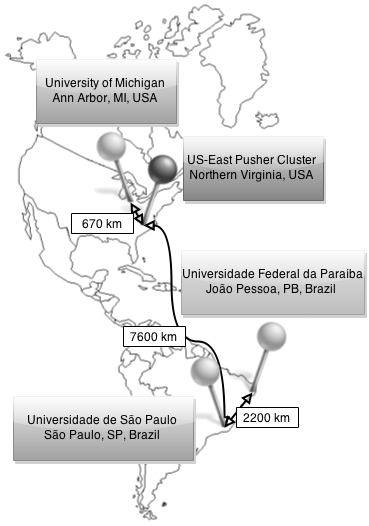
\includegraphics[width=0.4\columnwidth]{evaluation-routes-map-BW}
\caption{Routes between the universities with linear distance in kilometers}
\label{fig:routes}
\end{figure}


